\subsection{Тестирование производительности}

Производительность будет тестироваться с помощью встроенного в SolidWorks средства
SOLIDWORKS Performance Test. В этом тесте проверяется производительность системы в
типичных для SolidWorks задачах. Тестирование будет производиться на следующих
конфигурациях аппаратного обеспечения:
\begin{enumerate}
    \item Компьютеры, используемые на кафедре КПРС. Тест производится для оценки
        изначальной производительности системы.
    \item Используемый сервер. Включен в тест для оценки чистой производительности
        сервера, а также для оценки падения производительности на клиентских машинах.
    \item Разработанные тонкие клиенты. Тест проводится на 2 тонких клиентах и сервере
        одновременно для исследования влияния клиентов друг на друга. Тест отражает
        сценарий использования системы под нагрузкой.
    \item Тонкий клиент, тест запущен только на одном устройстве для верификации данных.
        Результаты должны быть идентичны пункту 2 (в пределах погрешности).
        Необходимо сравнить результаты с используемыми сейчас компьютерами для оценки
        изменения производительности всей системы.
\end{enumerate}

\begin{figure}[h]
    \center
    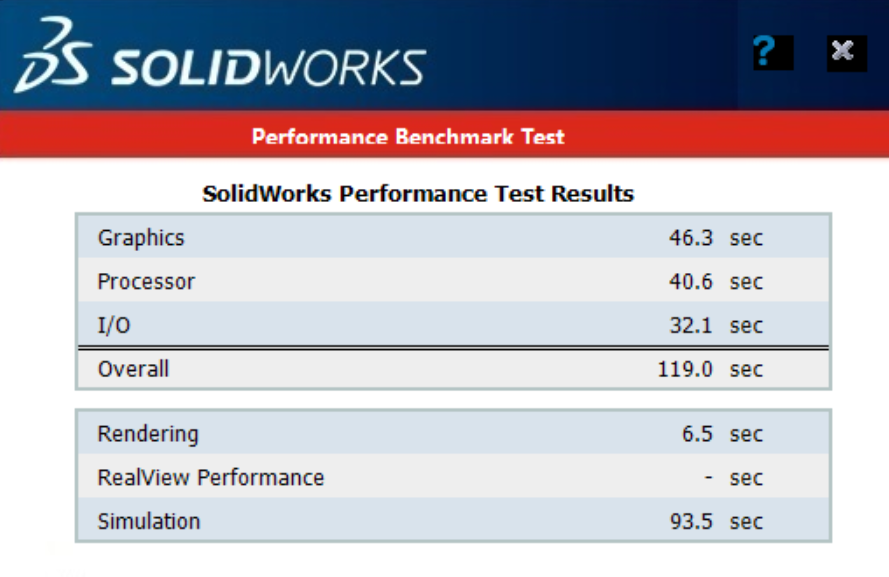
\includegraphics[height=9cm]{server_perf}
    \caption{Пример результата Solidworks Performance Test (2 конфигурация)}
    \label{pic:server_perf}
\end{figure}

Все тесты выполнялись 3 раза, результаты усреднены и представлены в сравнительной
таблице~\ref{tab:solid_comp}, а так же, для наглядности, на диаграмме (см.
рисунок~\ref{pic:solid_comp}). Данные показывают время выполнения одного теста и
представлены в секундах, меньше — лучше.

\begin{table}[h]
    \centering
    \caption{SOLIDWORKS Performance Test, средние значения}
    \label{tab:solid_comp}
    \begin{tabu}to \linewidth{XX[1,c,m]X[1,c,m]X[1,c,m]X[1,c,m]}
        \toprule
        Конфигурация & 1     & 2    & 3 & 4    \\
        \midrule
        Графика      & 52,1  & 48,3 &   & 46,5 \\
        Процессор    & 51,0  & 40,4 &   & 39,4 \\
        Ввод-вывод   & 31,7  & 30,8 &   & 33,0 \\
        Рендеринг    &  7,6  &  7,2 &   & 6,8  \\
        Симуляция    & 105,0 & 92,0 &   & 95,4 \\
        \bottomrule
    \end{tabu}
\end{table}

В целом тест показывает прирост производительности при переходе на систему тонких
клиентов. Однако, в ходе тестирования были обнаружены следующие проблемы:
\begin{itemize}
    \item На некоторых компьютерах тест не запускался, зависал во время выполнения или
        не выдавал результатов. 
    \item Разброс значений даже в пределах одного устройства достаточно высок, что не
        дает возможности сделать вывод на основании этого теста. 
\end{itemize}

Для подтверждения результатов общевычислительной производительности, будет произведено
дополнительное тестирование в программе PCMark 10, редакция Basic Edition
\cite{ref:pcmark}. 
Программы серии PCMark тестируют стабильность и производительность работы процессоров,
скоростные характеристики и пропускную способность оперативной и постоянной памяти, а
также множество других характеристик компьютерных компонентов. Для тестирования
используются различные тесты, как синтетические, нагружающие определённые блоки
компьютера, так и прикладные, например архивация данных, кодирование и декодирование
аудио и видео, производительность физического движка и т. д. 
PCMark является стандартом в индустрии компютерного аппаратного обеспечения.

Конфигурации тестируемого оборудования остались прежними, результаты тестирования
приведены в таблице~\ref{tab:pcmark_comp}. Результат для каждого теста выдается в виде
условных единиц, затем результаты всех тестов суммируются. Больше — лучше.

\begin{table}[h]
    \centering
    \caption{PCMark 10}
    \label{tab:pcmark_comp}
    \begin{tabu}to \linewidth{XX[1,c,m]X[1,c,m]X[1,c,m]X[1,c,m]}
        \toprule
        Конфигурация & 1     & 2    & 3 & 4    \\
        \midrule

        \midrule
        Итог &  &  &  &  \\
        \bottomrule
    \end{tabu}
\end{table}

Таким образом, по результатам проведенных тестов, можно сделать вывод о увеличении
производительности при использовании предложенной системы, состоящей из
производительного сервера и тонких клиентов в сценарии многопользовательской работы, по
сравнению с используемыми сейчас на кафедре компьютерами (толстыми клиентами). 
